\chapter{Event Displays
\label{ch:displays}}

\section{Leptoquark Search}

Figure \ref{fig:lq-evt1} shows the two-dimensional display in the transverse ($r$-$\phi$) plane and the three-dimensional display for the highest \ST observed event in the \mutau channel of the leptoquark search. Figure \ref{fig:lq-evt2} shows the same displays for the second-highest \ST observed event. The kinematic properties of the selected particles in those events are listed in Table \ref{tab:lq-evt}.

\begin{table}[htbp]
  \centering
    \begin{tabular}{|r|l|r|r|r|}
      \hline
      \multicolumn{1}{|c|}{\ST $[\GeVns]$} & \multicolumn{1}{c|}{Particle} & \multicolumn{1}{c|}{\pt $[\GeVns]$} & \multicolumn{1}{c|}{$\eta$} & \multicolumn{1}{c|}{$\phi$} \\
      \hline
      1444.6                               & $\mu$                         &   92.0                              & $-0.84$                     & $-0.16$ \\
                                           & \tauh                         &   87.8                              & $ 0.43$                     & $ 1.76$ \\
                                           & b-jet                         &  125.2                              & $ 1.63$                     & $ 1.57$ \\
                                           & jet                           & 1139.6                              & $-0.60$                     & $-2.72$ \\
      \hline
      1012.1                               & $\mu$                         &  293.6                              & $-0.49$                     & $-0.13$ \\
                                           & \tauh                         &   57.0                              & $ 0.37$                     & $-1.03$ \\
                                           & b-jet                         &   77.4                              & $ 1.92$                     & $-1.98$ \\
                                           & jet                           &  584.1                              & $-0.06$                     & $ 3.08$ \\
      \hline
    \end{tabular}
    \caption{The kinematic properties of the selected particles for the two highest \ST observed events in the \mutau channel of the leptoquark search.}    
    \label{tab:lq-evt}
\end{table}

\begin{figure}[hbtp]
\begin{center}
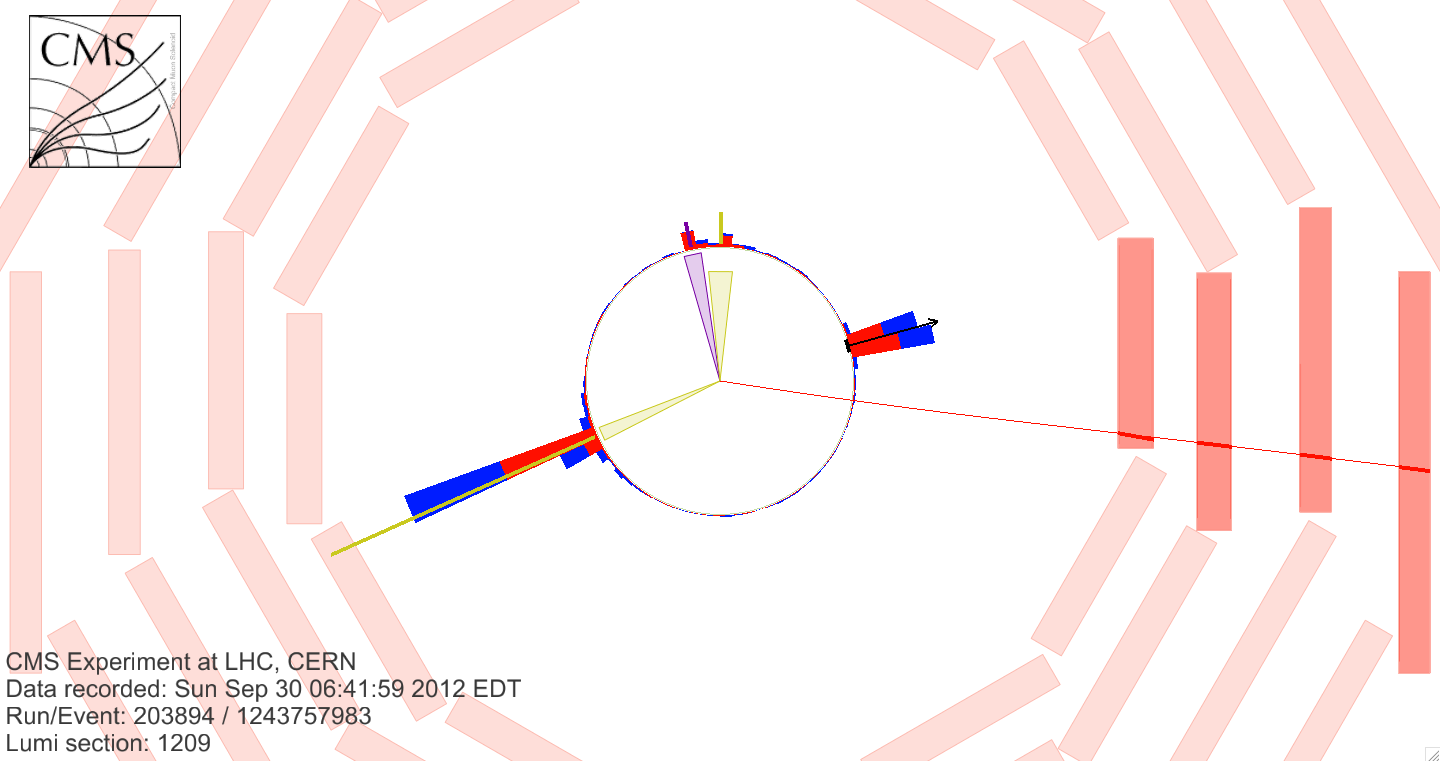
\includegraphics[width=0.95\textwidth]{figures/eventdisplays/LQ_evt1_rphi.png}
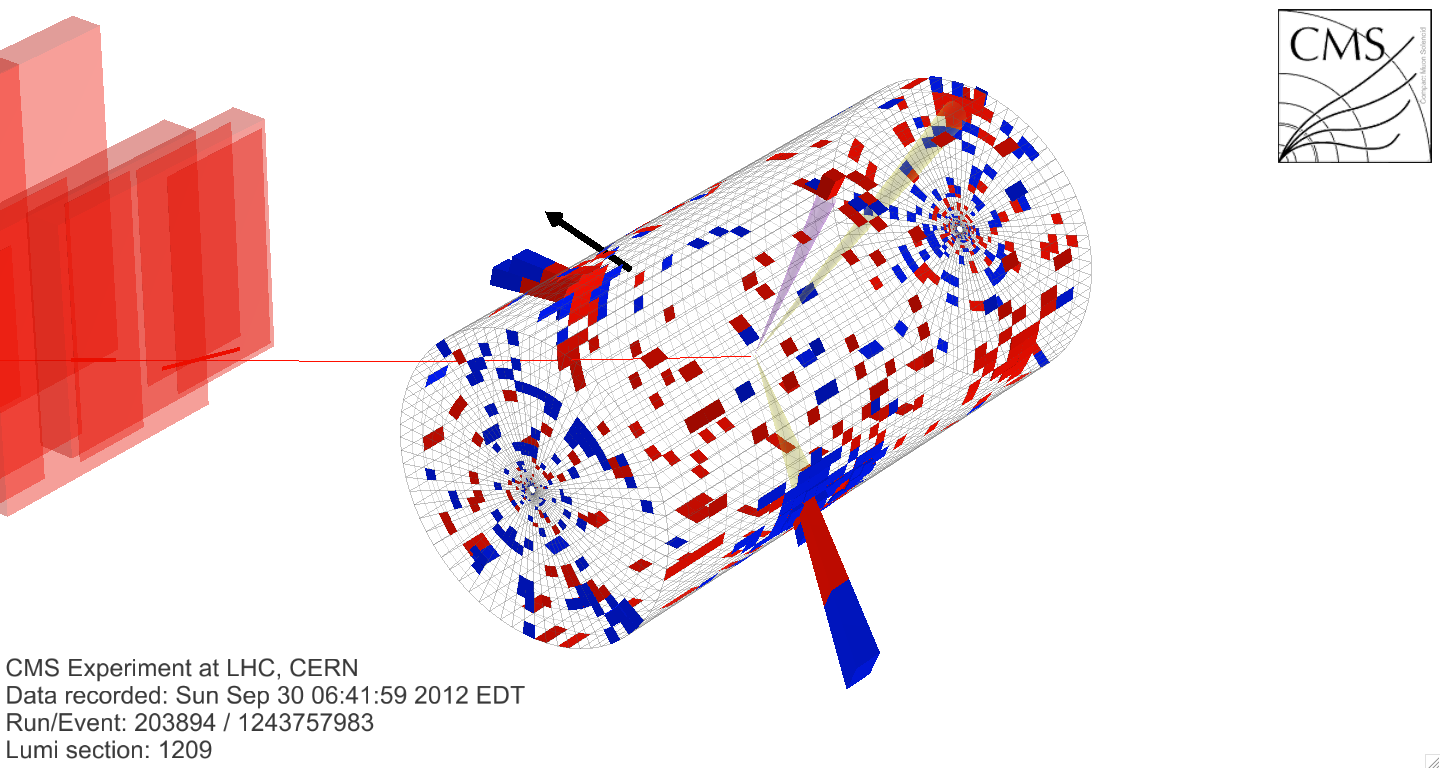
\includegraphics[width=0.95\textwidth]{figures/eventdisplays/LQ_evt1_3D.png}
\caption{A two-dimensional display in the transverse ($r$-$\phi$) plane (top) and a three-dimensional display (bottom) for the highest \ST observed event in the \mutau channel of the leptoquark search. The red line represents the muon, and the associated red rectangles represent the muon chamber hits. The purple cone represents the hadronic tau, and the yellow cones represent the jets. The black arrow indicates the \met in the event, while the ECAL and HCAL energy deposits are represented as red and blue towers, respectively. }
\label{fig:lq-evt1}
\end{center}
\end{figure}

\begin{figure}[hbtp]
\begin{center}
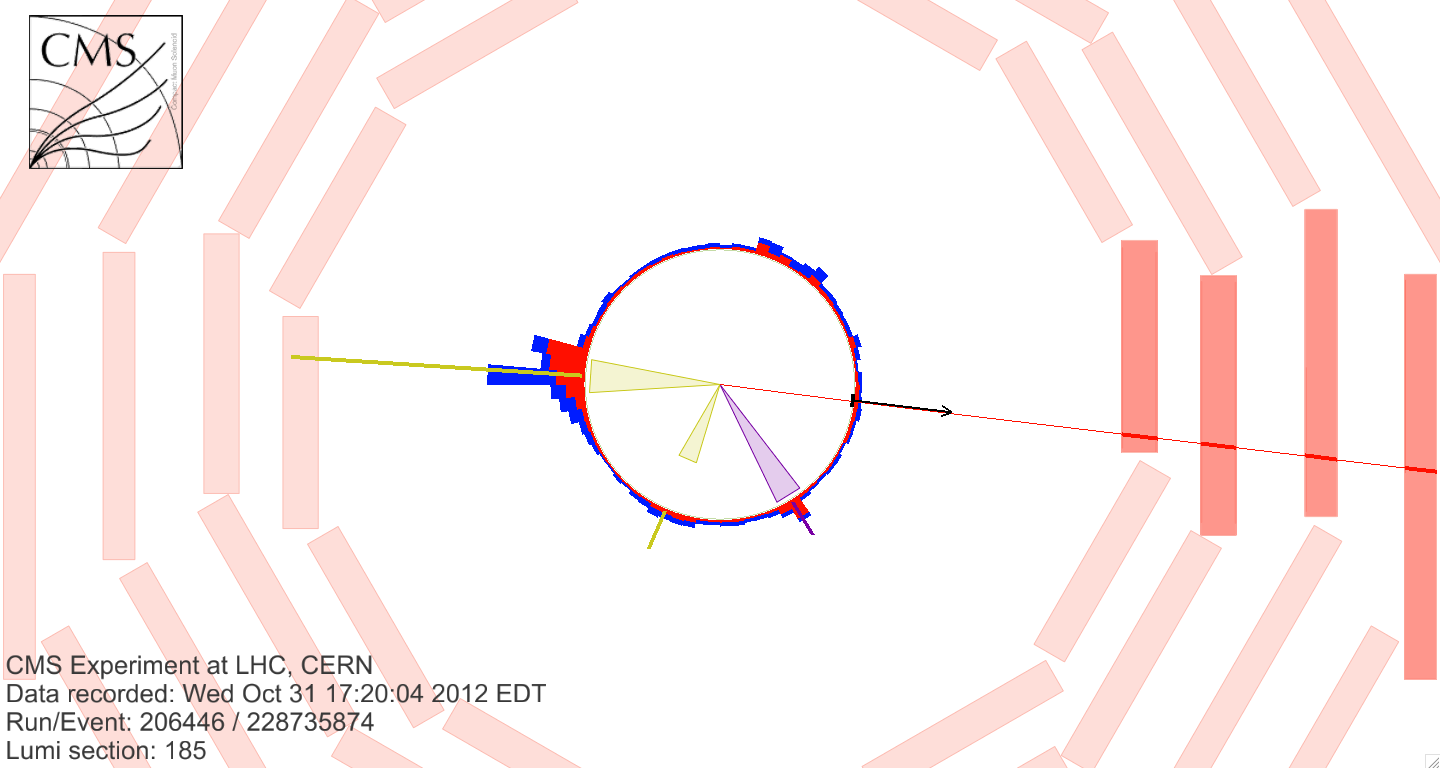
\includegraphics[width=0.95\textwidth]{figures/eventdisplays/LQ_evt2_rphi.png}
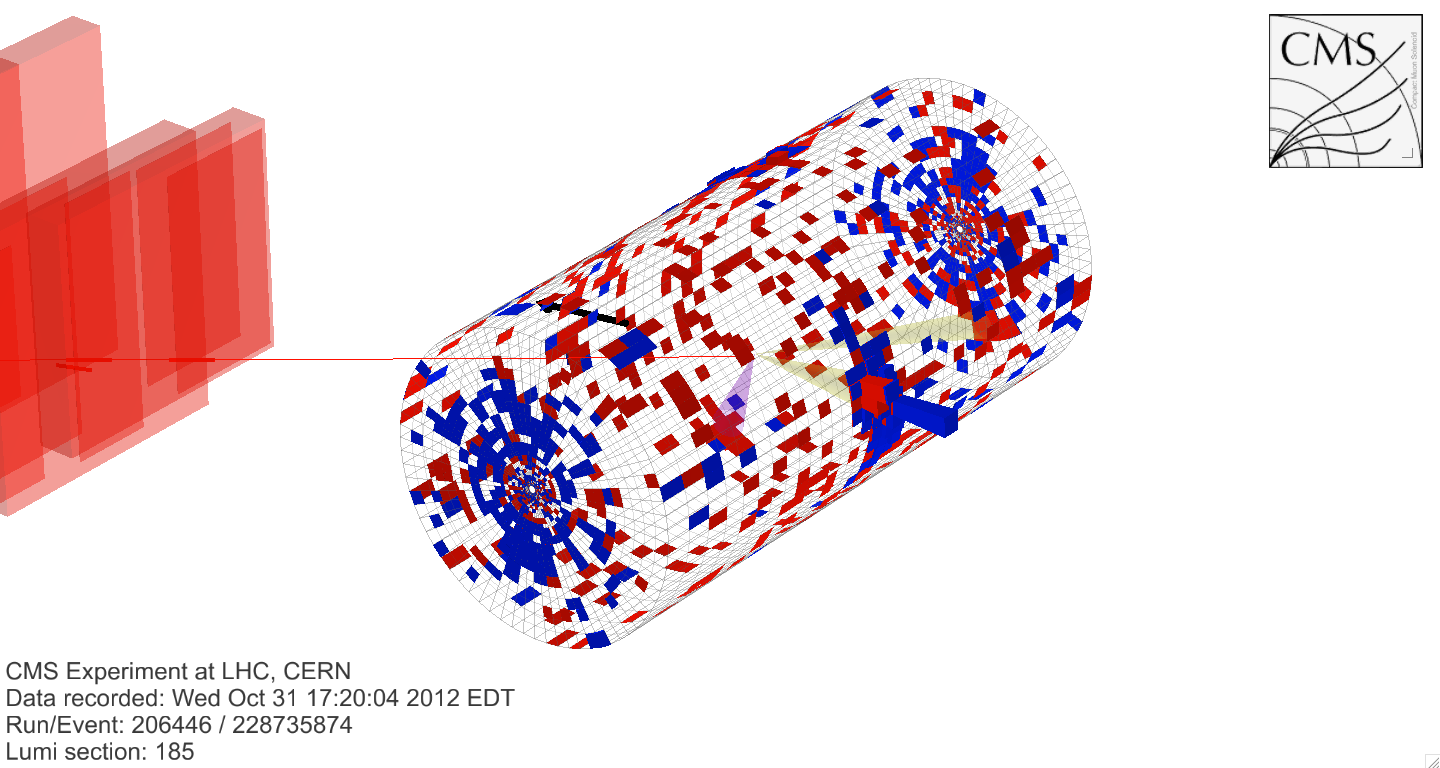
\includegraphics[width=0.95\textwidth]{figures/eventdisplays/LQ_evt2_3D.png}
\caption{A two-dimensional display in the transverse ($r$-$\phi$) plane (top) and a three-dimensional display (bottom) for the second-highest \ST observed event in the \mutau channel of the leptoquark search. The red line represents the muon, and the associated red rectangles represent the muon chamber hits. The purple cone represents the hadronic tau, and the yellow cones represent the jets. The black arrow indicates the \met in the event, while the ECAL and HCAL energy deposits are represented as red and blue towers, respectively. }
\label{fig:lq-evt2}
\end{center}
\end{figure}

\clearpage

\section{Top Squark Search}

Figure \ref{fig:lqd-evt1} shows the two-dimensional display in the transverse ($r$-$\phi$) plane and the three-dimensional display for the highest \ST observed event in the \mutau channel of the top squark search. Figure \ref{fig:lqd-evt2} shows the same displays for the second-highest \ST observed event. The kinematic properties of the selected particles in those events are listed in Table \ref{tab:lqd-evt}.

\begin{table}[htbp]
  \centering
    \begin{tabular}{|r|l|r|r|r|}
      \hline
      \multicolumn{1}{|c|}{\ST $[\GeVns]$} & \multicolumn{1}{c|}{Particle} & \multicolumn{1}{c|}{\pt $[\GeVns]$} & \multicolumn{1}{c|}{$\eta$} & \multicolumn{1}{c|}{$\phi$} \\
      \hline
      1586.2                               & $\mu$                         &   92.0                              & $-0.84$                     & $-0.16$ \\
                                           & \tauh                         &   87.8                              & $ 0.43$                     & $ 1.76$ \\
                                           & b-jet                         &  125.2                              & $ 1.63$                     & $ 1.57$ \\
                                           & jet 1                         & 1139.6                              & $-0.60$                     & $-2.72$ \\
                                           & jet 2                         &   63.5                              & $-0.05$                     & $-2.77$ \\
                                           & jet 3                         &   42.9                              & $ 1.10$                     & $-2.87$ \\
                                           & jet 4                         &   35.2                              & $-1.69$                     & $-2.19$ \\
      \hline
      1136.3                               & $\mu$                         &  313.1                              & $-0.09$                     & $-1.18$ \\
                                           & \tauh                         &   53.7                              & $ 1.83$                     & $ 0.89$ \\
                                           & b-jet                         &  156.0                              & $-0.09$                     & $ 1.52$ \\
                                           & jet 1                         &  325.3                              & $ 0.00$                     & $ 2.49$ \\
                                           & jet 2                         &  123.1                              & $-0.67$                     & $-1.57$ \\
                                           & jet 3                         &  103.0                              & $-0.59$                     & $ 1.93$ \\
                                           & jet 4                         &   62.2                              & $-0.62$                     & $-2.32$ \\
      \hline
    \end{tabular}
    \caption{The kinematic properties of the selected particles for the two highest \ST observed events in the \mutau channel of the top squark search.}    
    \label{tab:lqd-evt}
\end{table}

\begin{figure}[hbtp]
\begin{center}
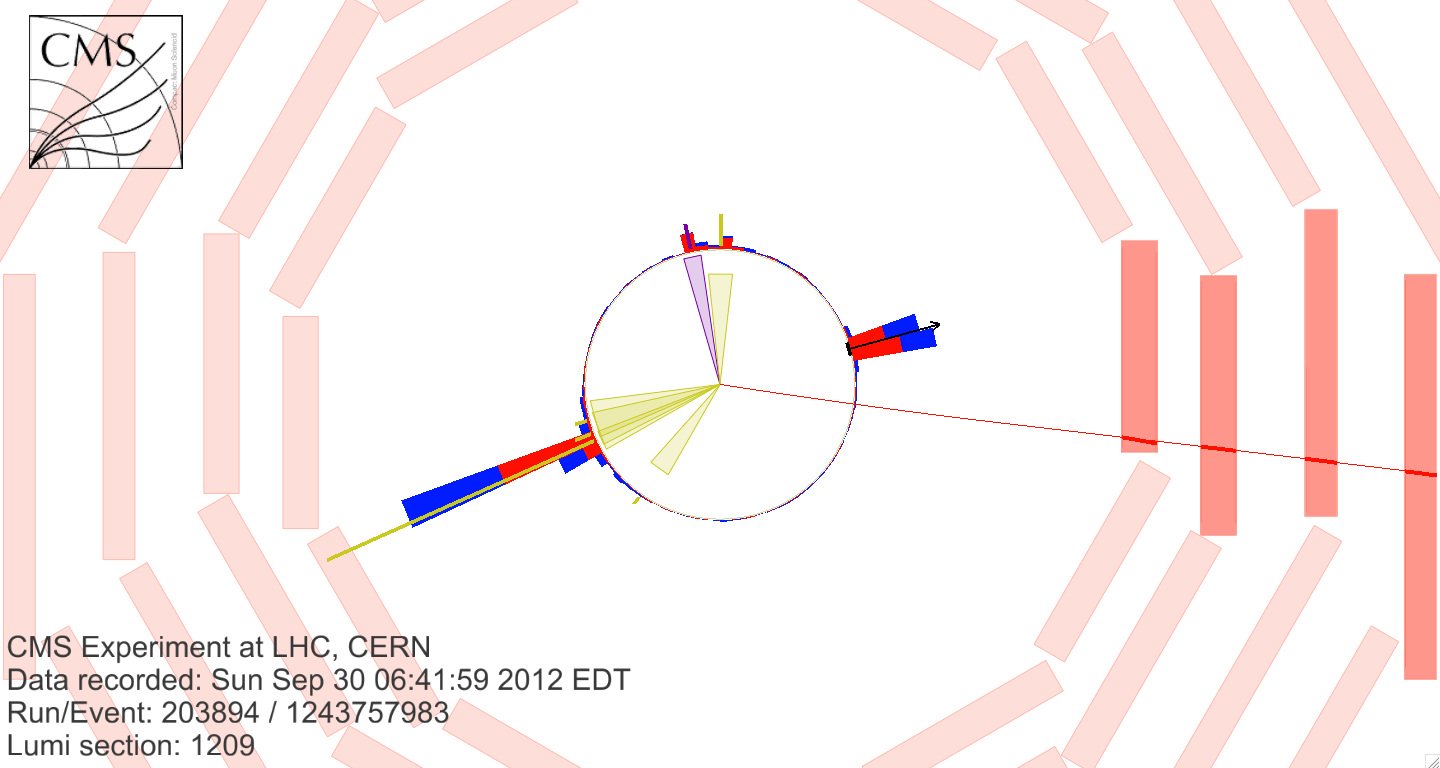
\includegraphics[width=0.95\textwidth]{figures/eventdisplays/LQD_evt1_rphi.png}
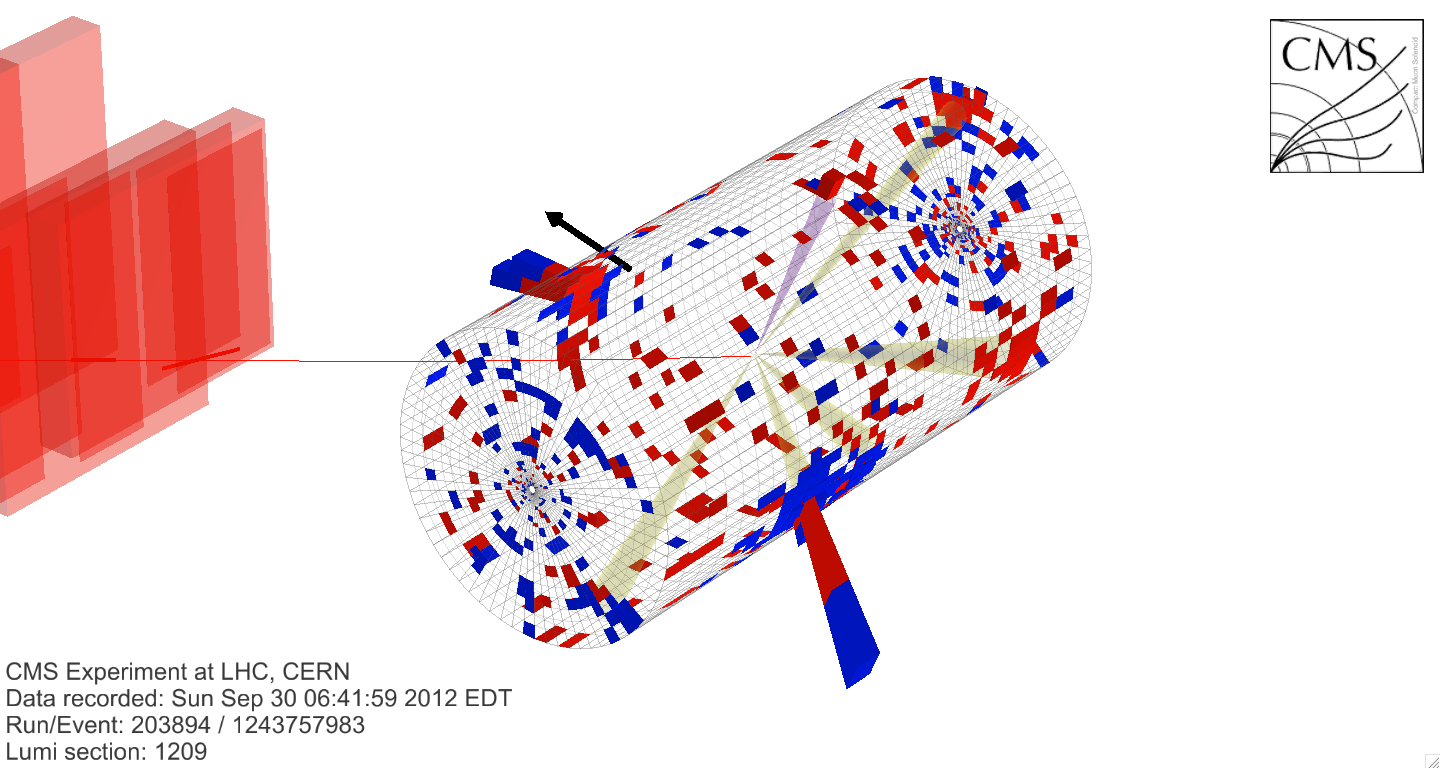
\includegraphics[width=0.95\textwidth]{figures/eventdisplays/LQD_evt1_3D.png}
\caption{A two-dimensional display in the transverse ($r$-$\phi$) plane (top) and a three-dimensional display (bottom) for the highest \ST observed event in the \mutau channel of the top squark search. The red line represents the muon, and the associated red rectangles represent the muon chamber hits. The purple cone represents the hadronic tau, and the yellow cones represent the jets. The black arrow indicates the \met in the event, while the ECAL and HCAL energy deposits are represented as red and blue towers, respectively. }
\label{fig:lqd-evt1}
\end{center}
\end{figure}

\begin{figure}[hbtp]
\begin{center}
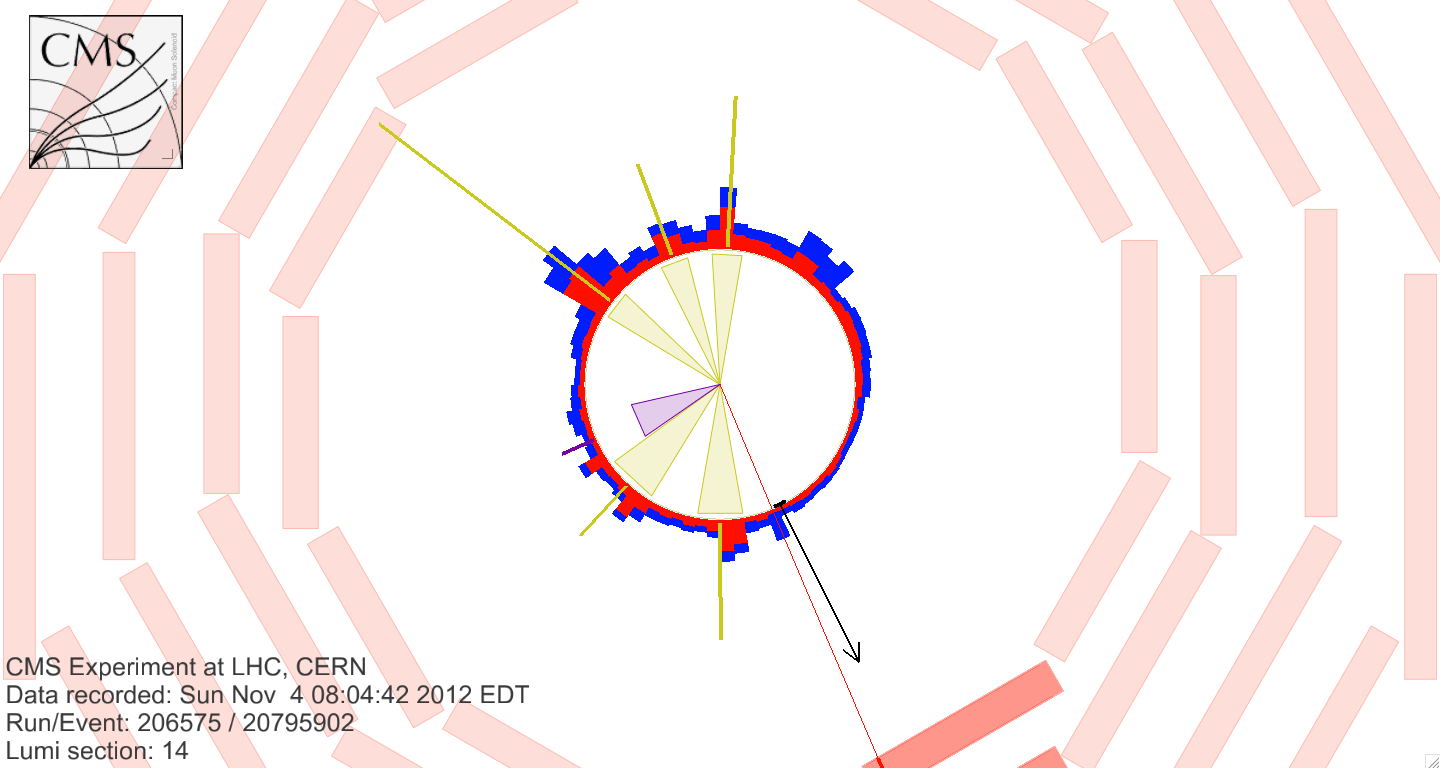
\includegraphics[width=0.95\textwidth]{figures/eventdisplays/LQD_evt2_rphi.png}
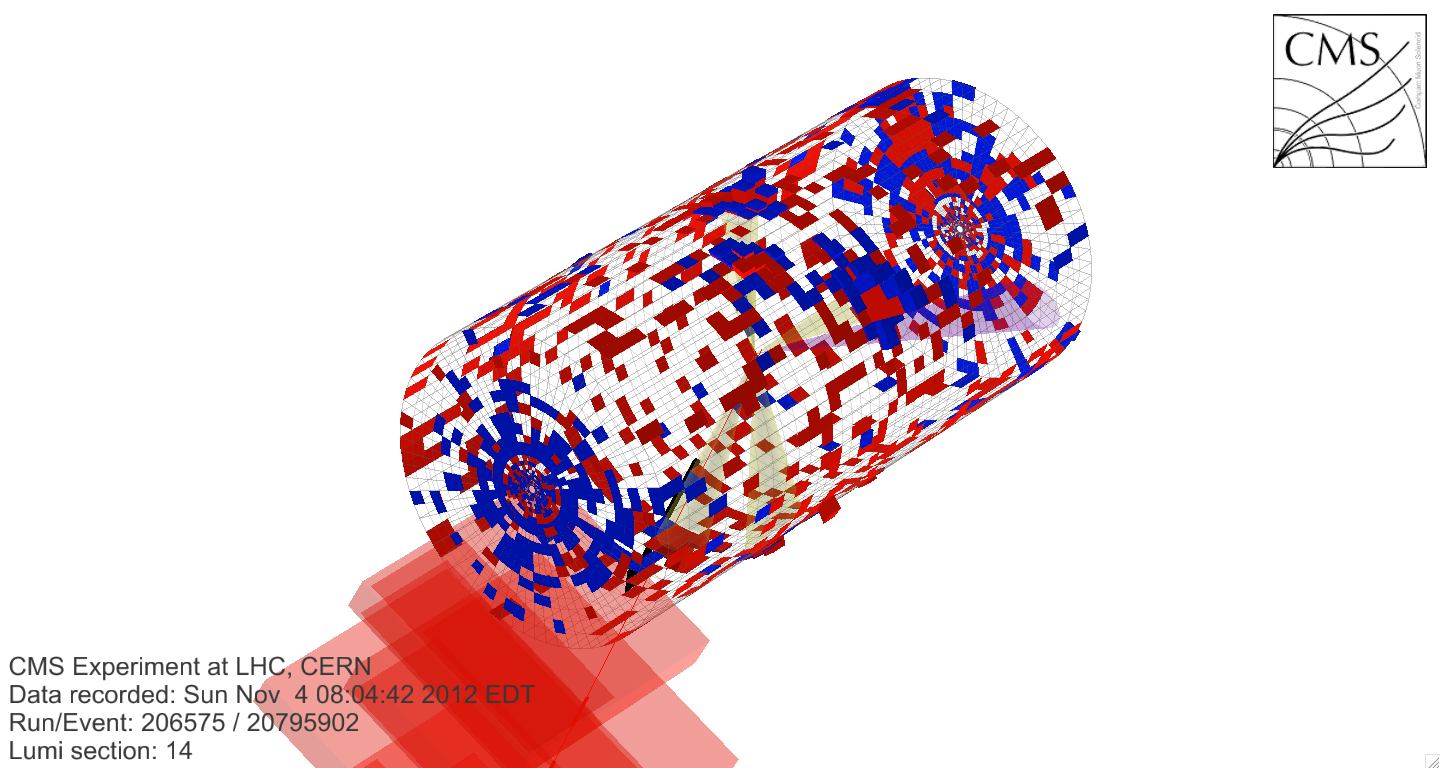
\includegraphics[width=0.95\textwidth]{figures/eventdisplays/LQD_evt2_3D.png}
\caption{A two-dimensional display in the transverse ($r$-$\phi$) plane (top) and a three-dimensional display (bottom) for the second-highest \ST observed event in the \mutau channel of the top squark search. The red line represents the muon, and the associated red rectangles represent the muon chamber hits. The purple cone represents the hadronic tau, and the yellow cones represent the jets. The black arrow indicates the \met in the event, while the ECAL and HCAL energy deposits are represented as red and blue towers, respectively. }
\label{fig:lqd-evt2}
\end{center}
\end{figure}